\section{Web Application}\label{methodology}

We also build a web application to interact with users. Our web application structure is shown in figure \ref{structure}. We use Node JS as web framework. For each new UFO sighting report data, we will call detection program to check it, produce truth possibility. Based on grading, we will assign true (1) or fake (0) to the report, and update my\_ufo.db. The system will periodically redo model training process based on all report data.

\begin{figure}[H]
    \centering
    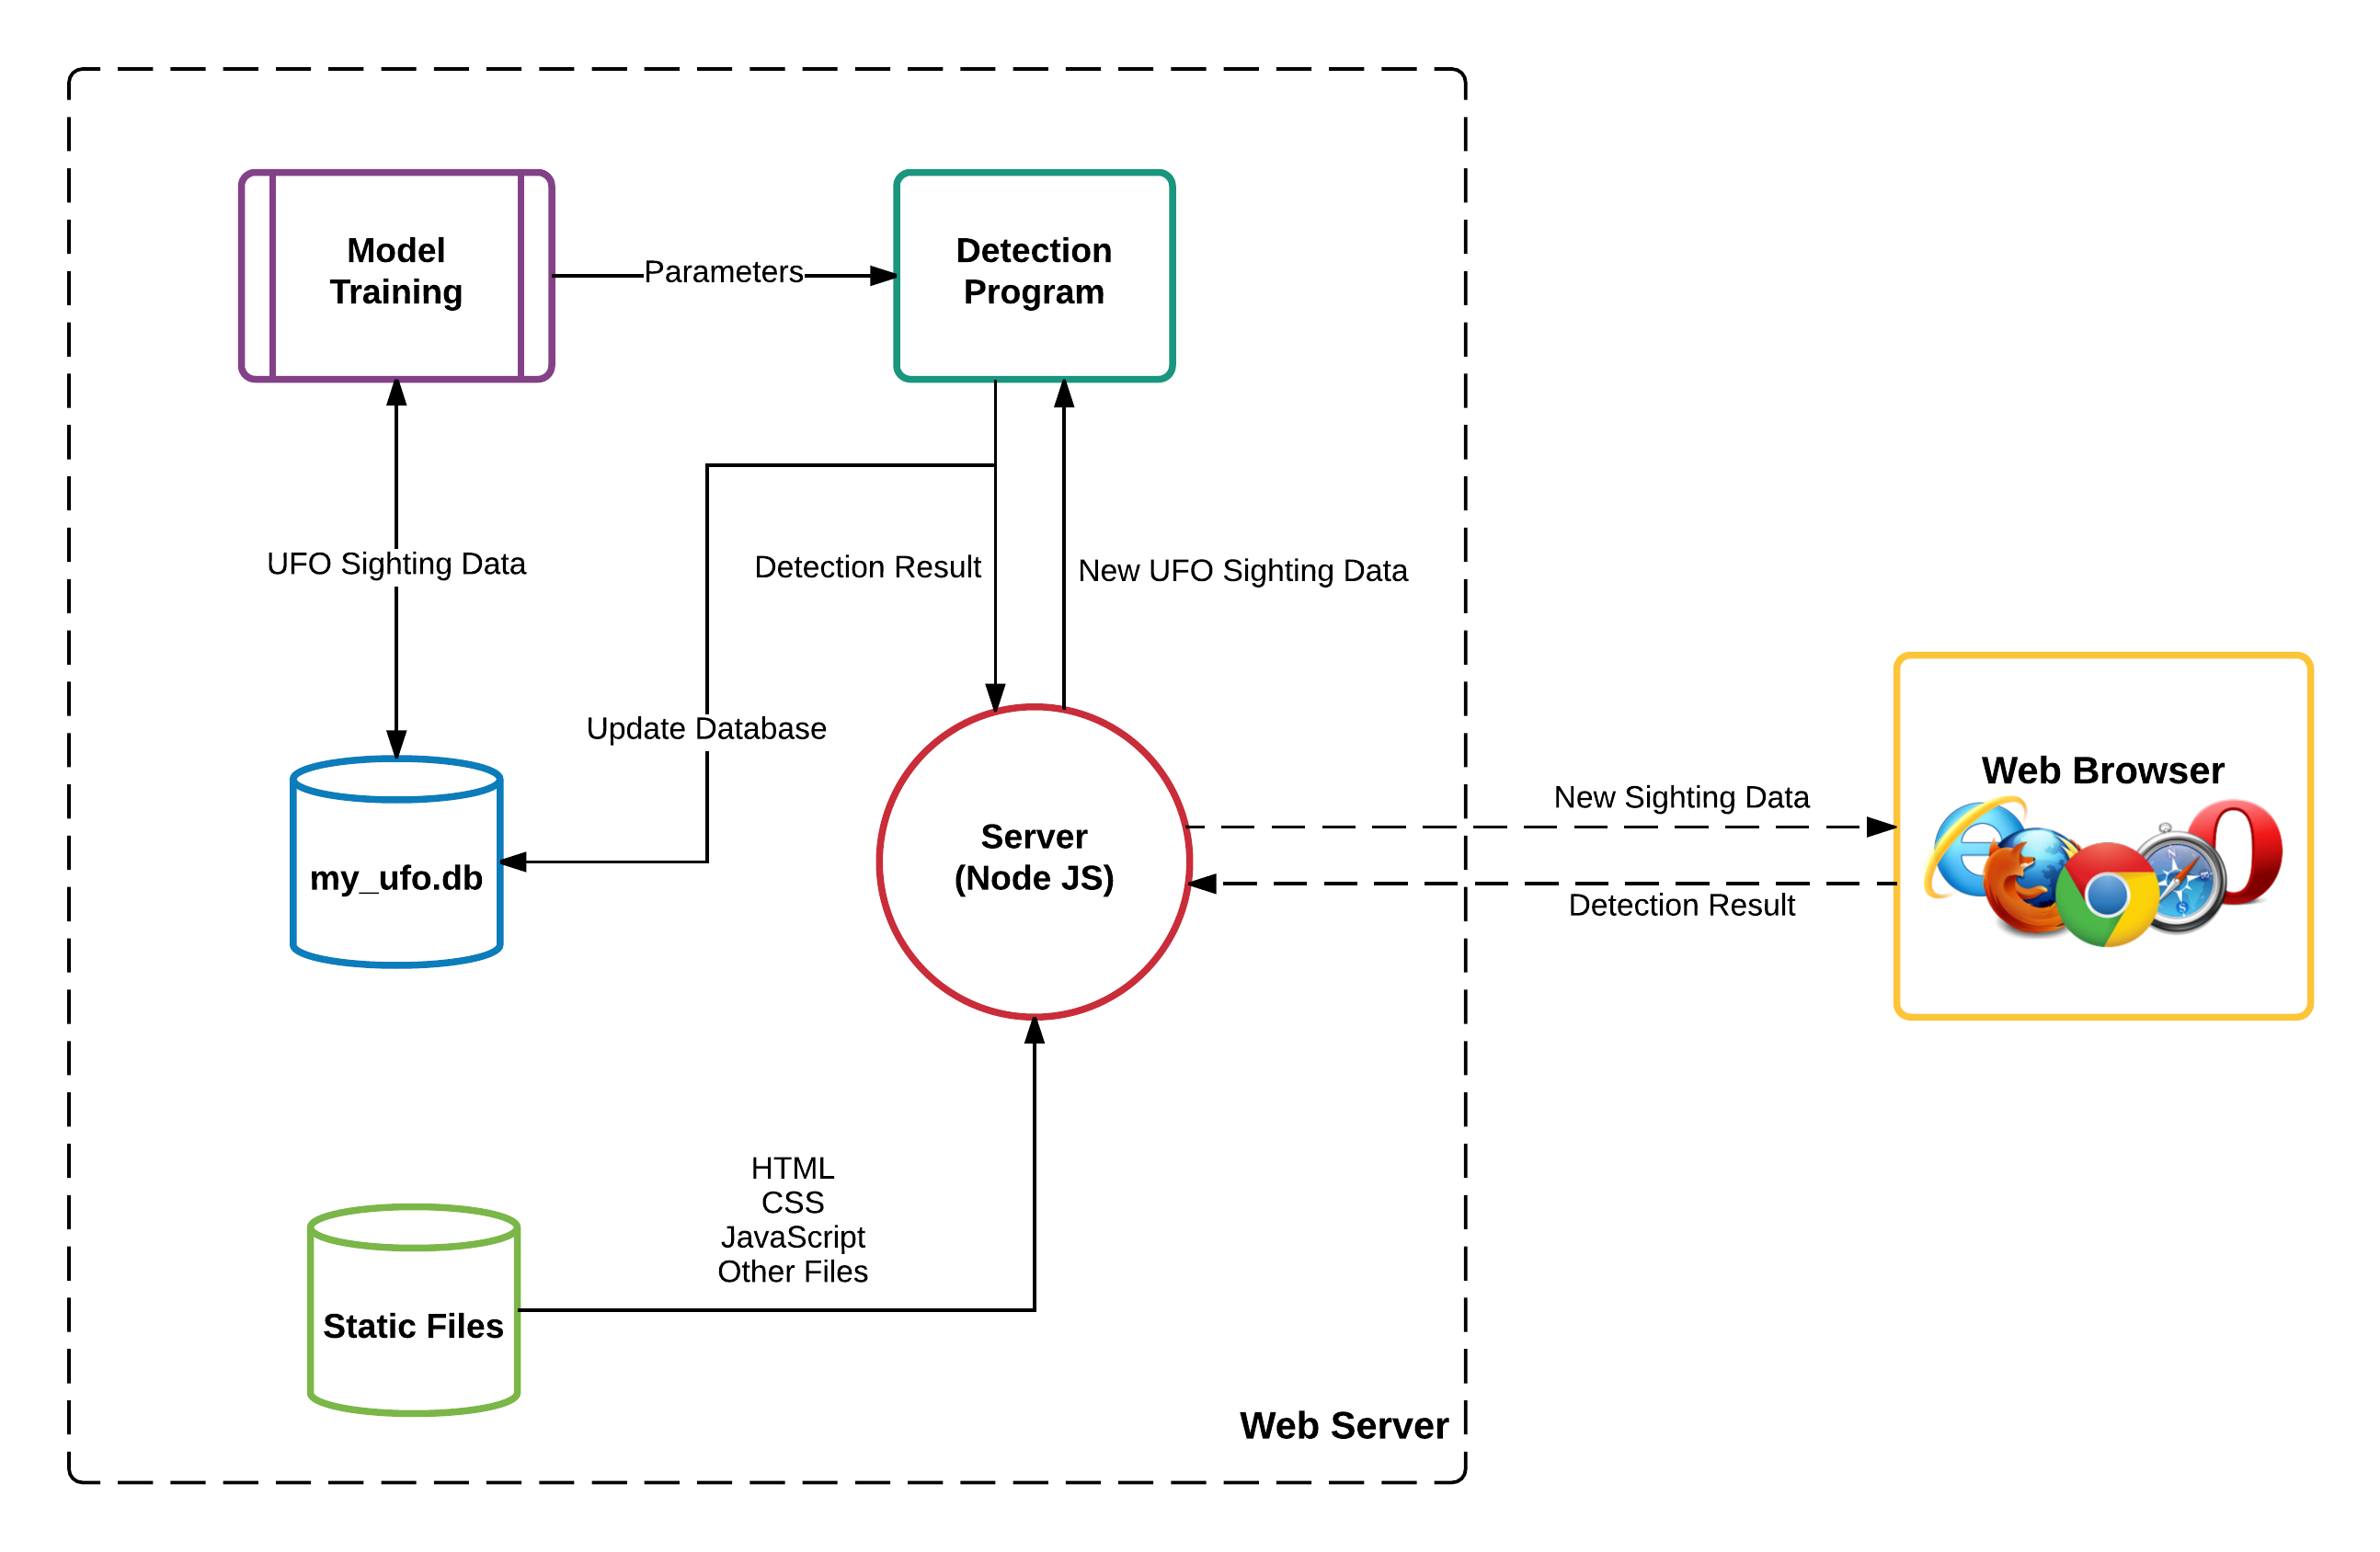
\includegraphics[width=12cm]{figure/structure.png}
    \caption{web structure}
    \label{structure}
\end{figure}

\begin{figure}
\centering 
\subfigure[home page]{\label{home}
\begin{minipage}[b]{0.6\textwidth}
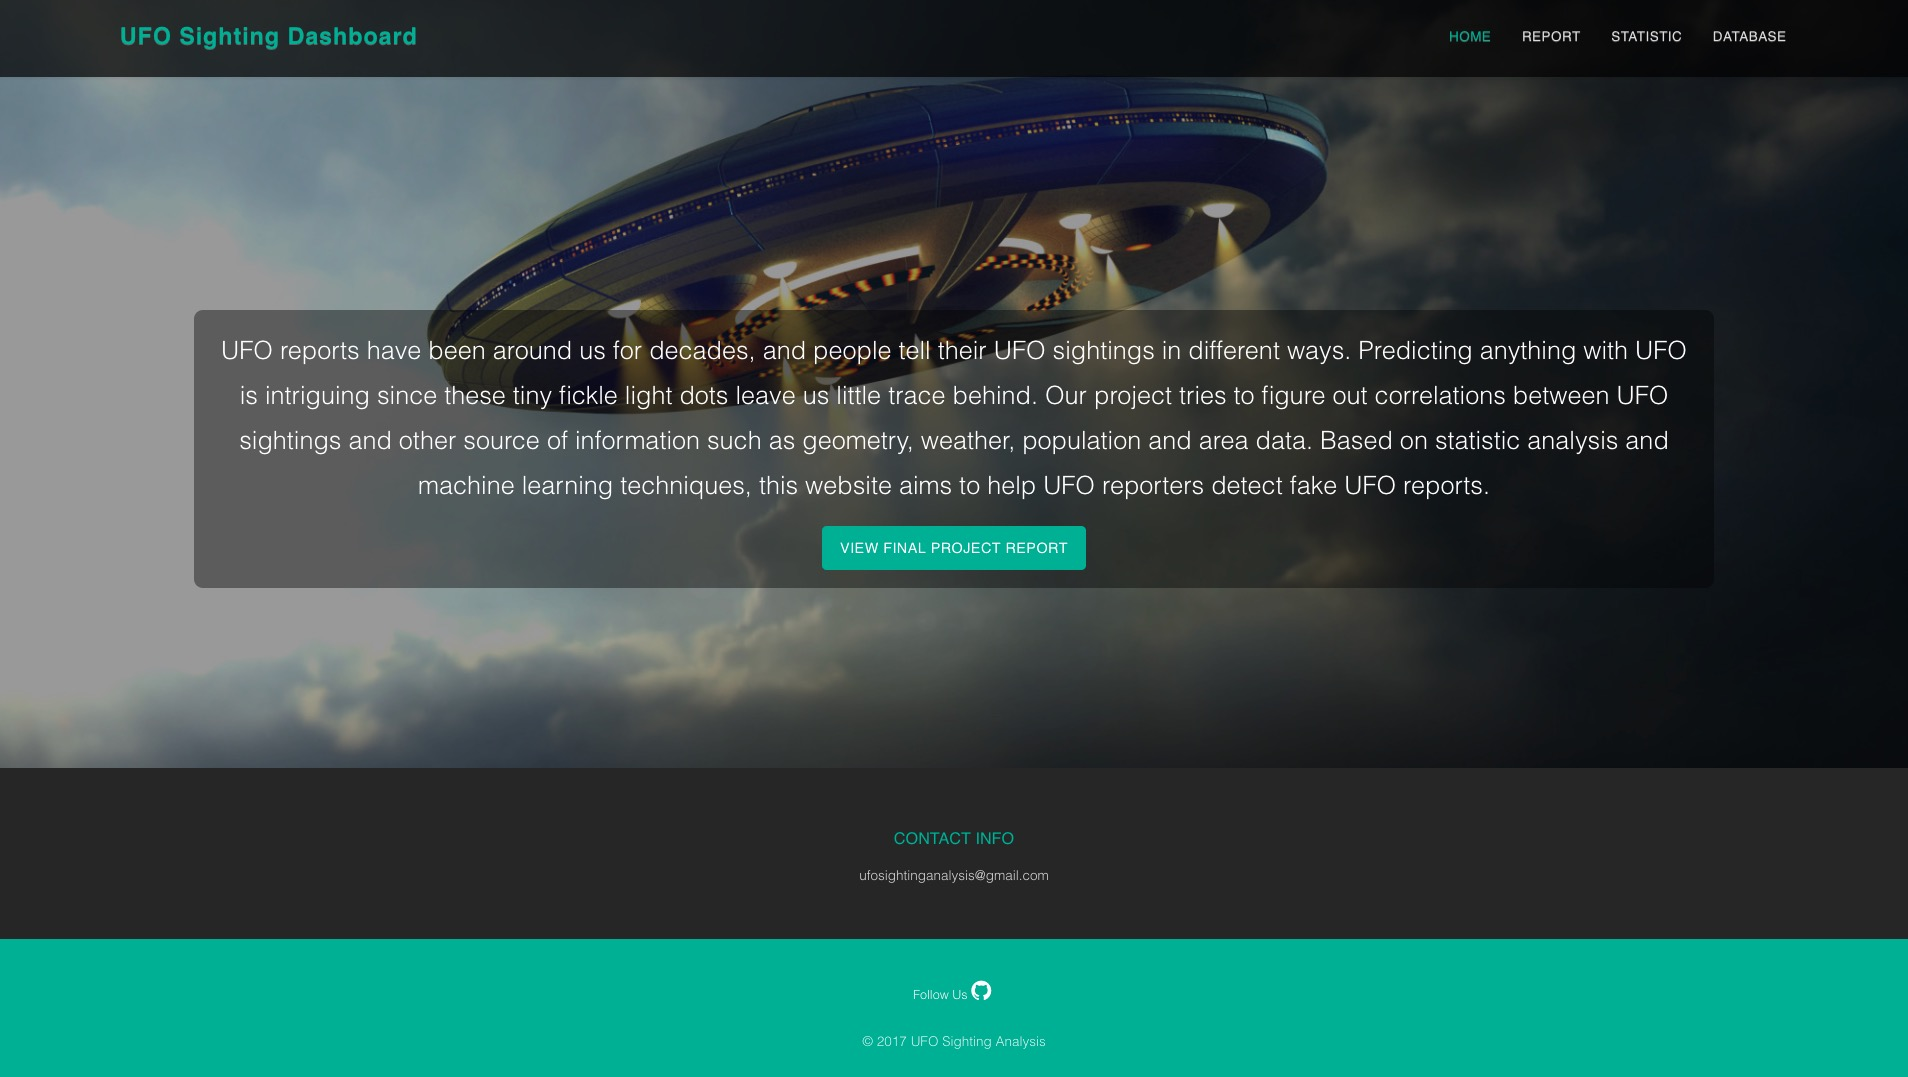
\includegraphics[width=1\textwidth]{figure/home.jpg}
\end{minipage}
}
\subfigure[statistic page]{\label{stats}
\begin{minipage}[b]{0.6\textwidth}
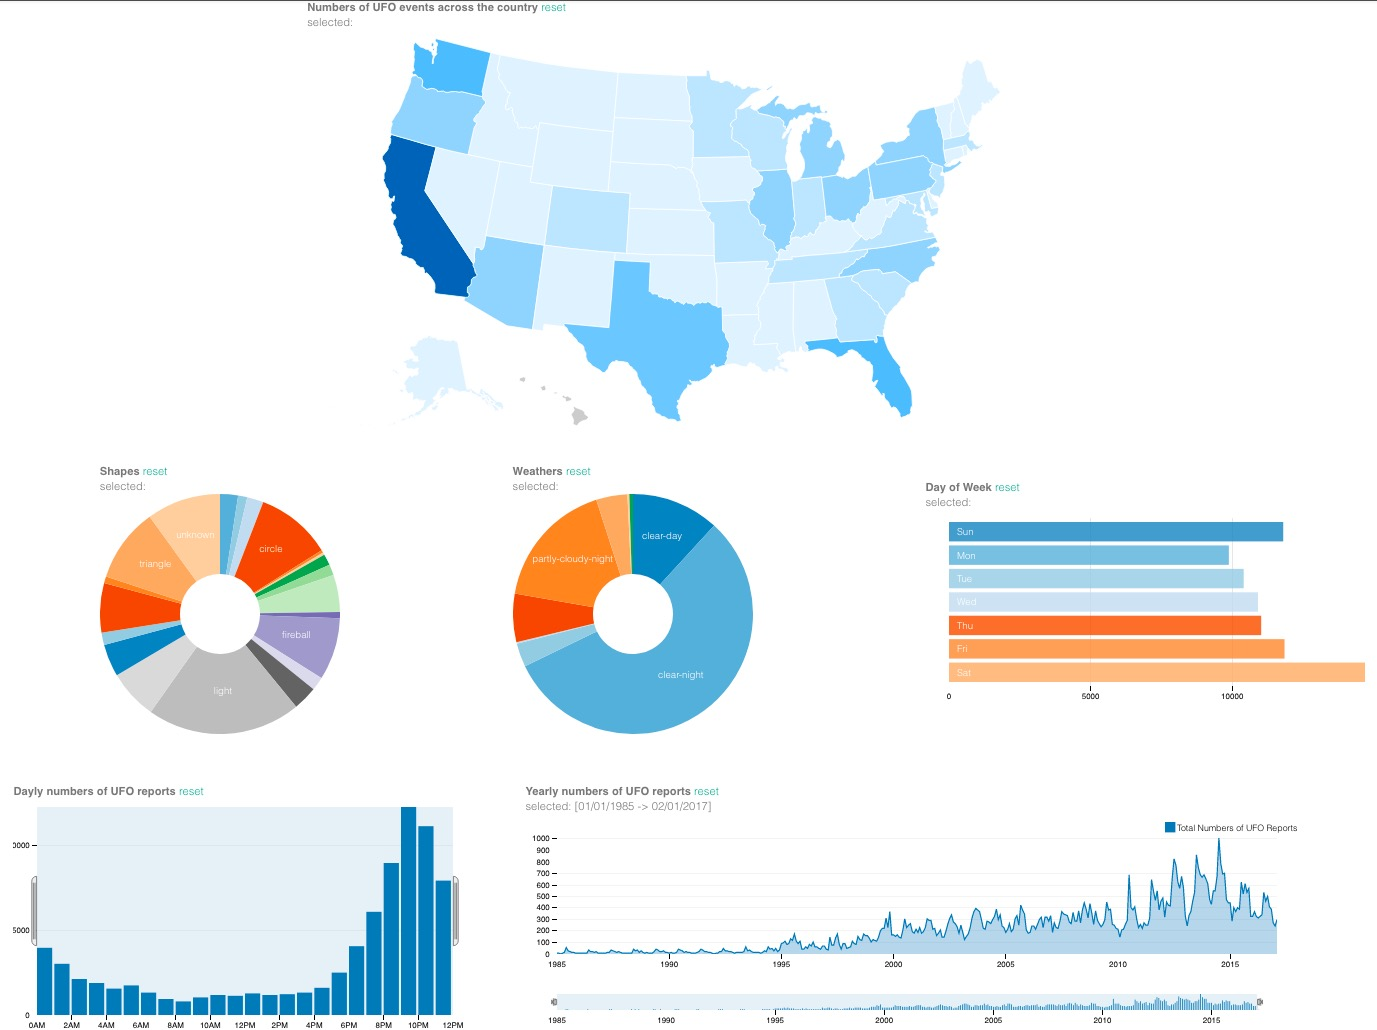
\includegraphics[width=1\textwidth]{figure/statistic.jpg}
\end{minipage}
}
\subfigure[database page]{\label{database}
\begin{minipage}[b]{0.6\textwidth}
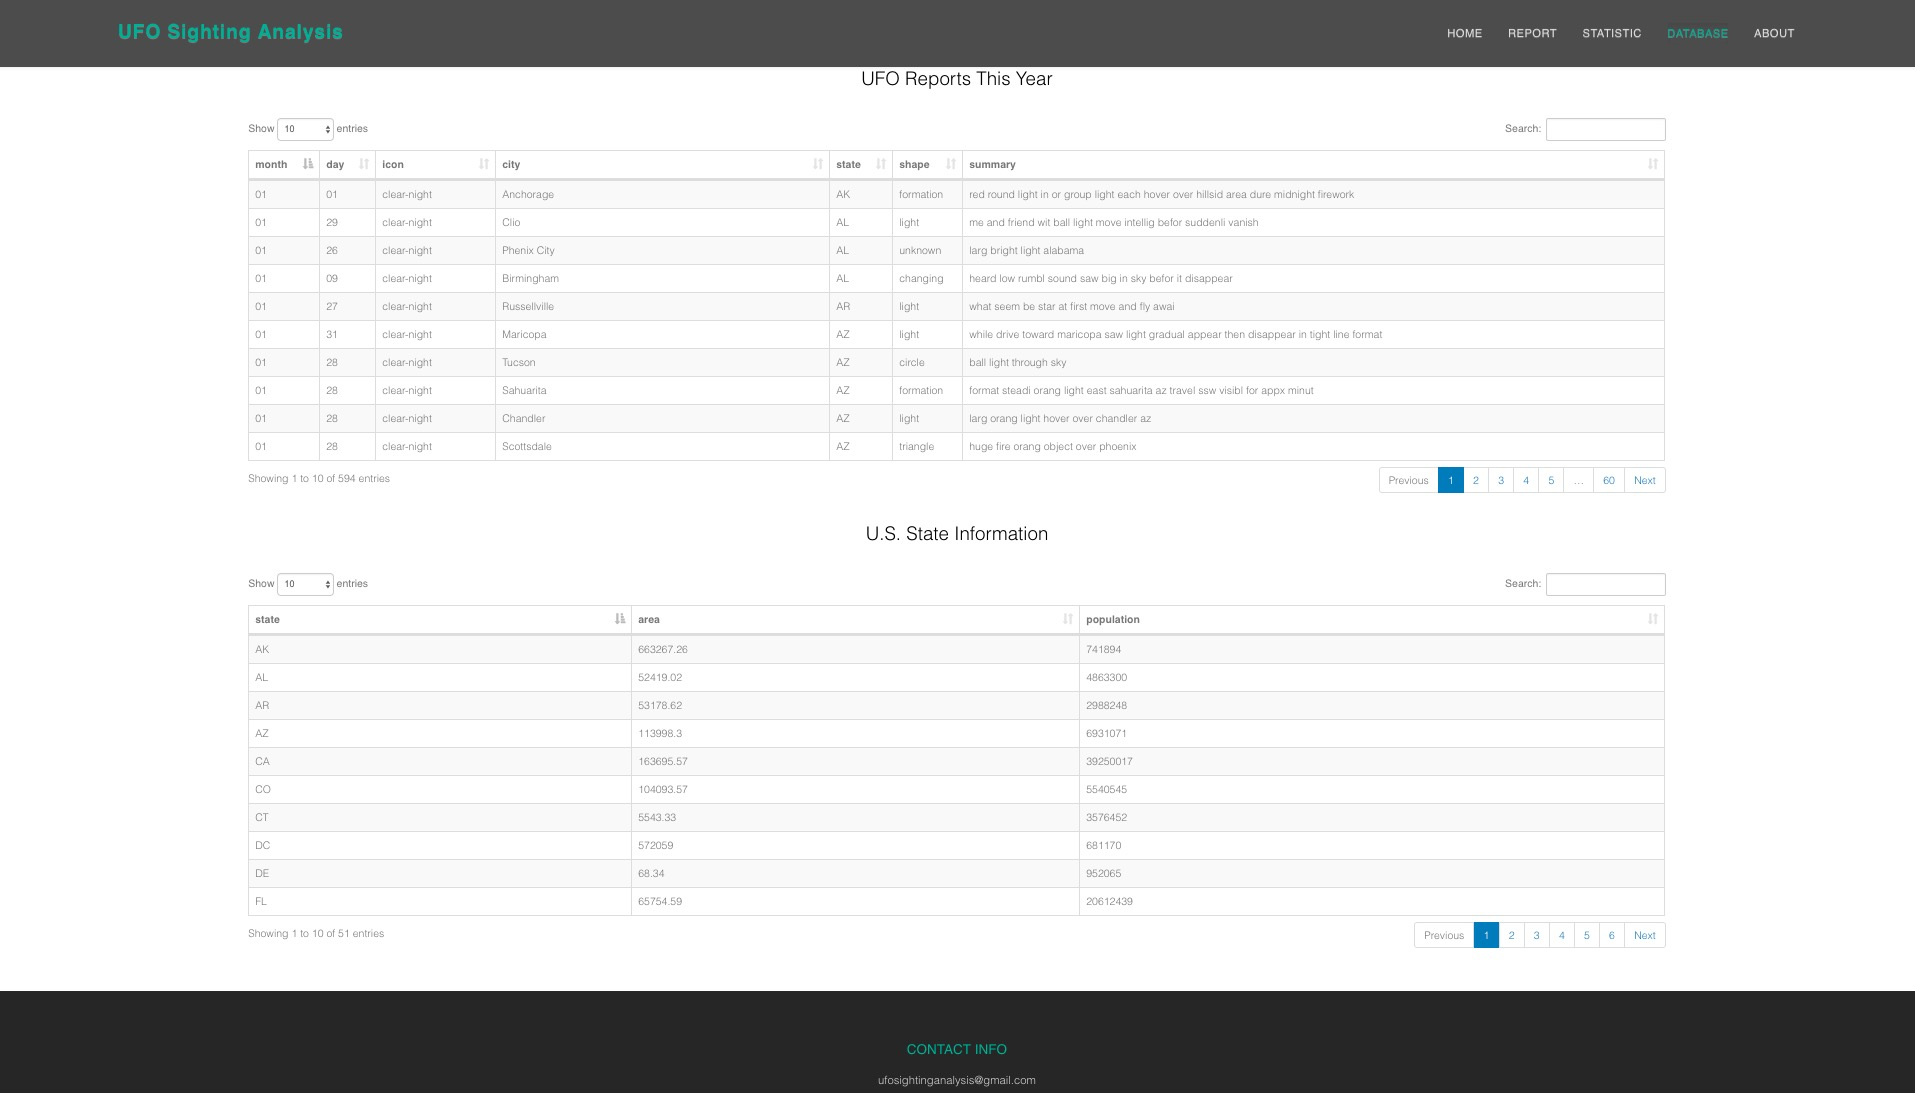
\includegraphics[width=1\textwidth]{figure/database.jpg}
\end{minipage}
}
\caption{home, statistic and database page}
\end{figure}

The home page of our website is shown in figure \ref{home}. There are three major functions of our website --- reporting UFO sighting, viewing statistic results, viewing database. Report page displayed in figure \ref{report} requires users to enter some information about their sightings: where, when, how long, what shape and their own summary. By clicking complete button, we will gather their reports' data and calculate their credibility by machine learning model illustrated in section \ref{ml}. Figure \ref{feedback} is a possible feedback to users. The classifier result is the possibility calculated by four classifiers separately. They vote in average to give out the final grade of user report. Numeric information lists other numeric features we gained from their report information. Information contribution is the proportion of grades between numeric and summary classifiers:
$$
sum\_log + sum\_tree : num\_svm + num\_tree
$$
Finally, we mark out user sighting against the accumulative UFO sighting distribution around U.S in a heat map. 



\begin{figure}[H]
\centering 
\subfigure[report page]{\label{report}
\begin{minipage}[b]{0.8\textwidth}
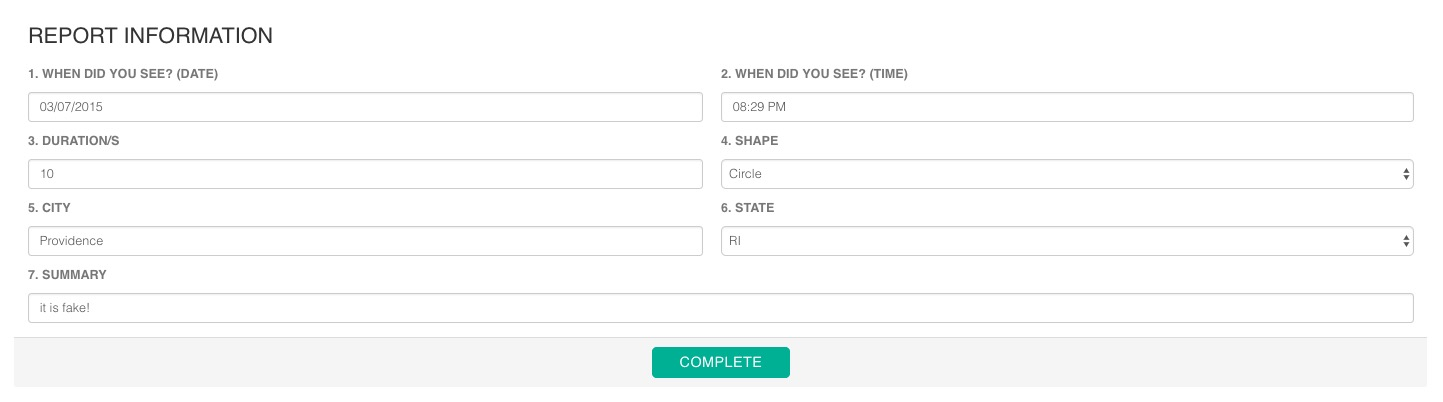
\includegraphics[width=1\textwidth]{figure/report.jpg}
\end{minipage}
}
\subfigure[feedback]{\label{feedback}
\begin{minipage}[b]{0.8\textwidth}
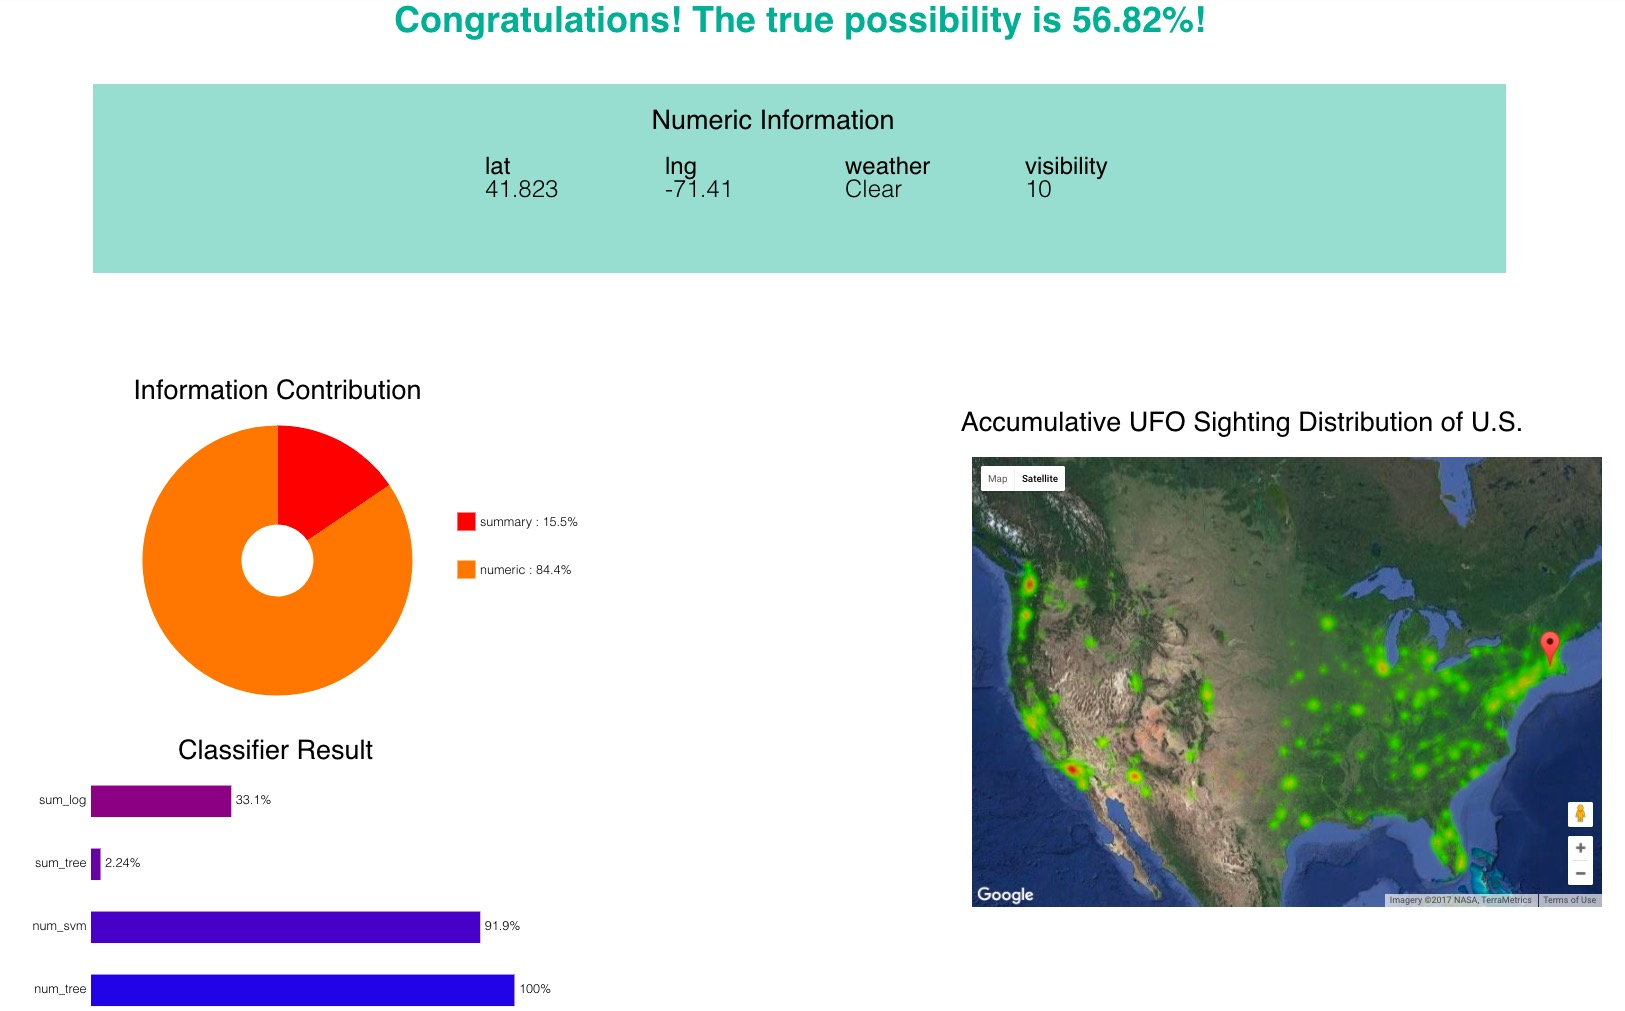
\includegraphics[width=1\textwidth]{figure/feedback.jpg}
\end{minipage}
}
\caption{report page}
\end{figure}

Statistic page in figure \ref{stats} shows our analysis results described in section \ref{statistic}. We use crossfilter~\cite{dcjs} to provide instant feedback to user interaction. Database view exhibits in figure \ref{database} uses DataTable~\cite{datatable} To show UFO reports in current year, as well as population and area information of U.S. that we used for machine learning.
